\documentclass[12pt]{report}
\usepackage[utf8]{inputenc}
\usepackage[english]{babel}
\usepackage{csquotes}
\usepackage{amssymb}
\usepackage{amsmath}
\usepackage{mathrsfs}
\usepackage{tikz}
\usepackage{pgfplots}
\pgfplotsset{compat=1.7}
\usepackage[a4paper,left=3cm,right=2cm,top=2.5cm,bottom=2.5cm]{geometry}
\usepackage{marginnote}
\usepackage[makeroom]{cancel}

\usepackage[
    backend=biber,
    style=alphabetic,
    sorting=ynt
]{biblatex}

\addbibresource{mybib.bib} %Imports local bibliography file



\title{Master Thesis}
\author{Alberto Tiraboschi}
%\date{ }

\begin{document}

\numberwithin{equation}{section}

\maketitle
\cleardoublepage

\tableofcontents
\cleardoublepage

Expected 40 pgg everything included
\chapter{Example citing}

Using \texttt{biblatex} you can display bibliography divided into sections, depending of citation type. 
Let's cite! Einstein's journal paper \cite{friis_m} and the Dirac's book \cite{dirac} are physics related items. Also Einstein \cite{einstein}. Next, \textit{The \LaTeX\ Companion} book \cite{latexcompanion}, the Donald Knuth's website \cite{knuthwebsite}, \textit{The Comprehensive Tex Archive Network} (CTAN) \cite{ctan} are \LaTeX\ related items; but the others Donald Knuth's items \cite{knuth-fa,knuth-acp} are dedicated to programming. 
\clearpage

\chapter{Abstract, possibili applicazioni, descrizione (1 pg)}
\clearpage

\chapter{Modello matematico della propagazione del segnale (2 pag)}
\section{Path loss model}
From \cite{friis_m}...

\begin{equation}
RSSI(d) = A-10\alpha\log\bigg(\frac{d}{d_0}\bigg)    
\end{equation}

where $A$ is the $RSSI$ read at $d_0$. Commonly $d_0$ is taken as $1$ meter, so that 

\begin{equation}
RSSI(d) = A-10\alpha\log(d_0)    
\end{equation}
$\alpha$ is the path loss index, which can vary between $2$ (open field) and $4$ (environment fitted with obstacles).
\clearpage


\chapter{Alterazioni della misura dovute all'ambiente (3 pag)}
\section{Descrizione}
\section{Analisi probailistica degli algoritmi errore uniforme}
https://github.com/pspachos/RSSI-Dataset\\
$https://www.jmp.com/en_us/statistics-knowledge-portal/chi-square-test/chi-square-goodness-of-fit-test.html$
\section{Methods to remove outliers}
IQR, Z score

\clearpage



\chapter{Algoritmi (15 pag)}
scrivere vantaggi e svantaggi ognuno, testo algoritmo, dimostrazioni matematiche, commenti e opinioni.
\section{General overview and recurring terms}
We want to locate a device, (with a LOS or NLOS condition ?) by exploiting the relation between the received signal strength and the distance between the source node and the position where the measurement is taken. In real scenarios these samples can be provided mainly in two ways. One typical way is to place various anchor nodes, such that the anchor node $i$, can give samples like $(x_i,y_i,rssi_i)$. The other way, which is lately becoming increasingly used is the employment of a drone, that given some bounds on the area to scan, it collects and outputs the samples, behaving as a "moving" anchor node.
\section{Recurring terms}
We have $n$ anchor nodes with known position, and a $t$-th target node with unknown position.The anchor node $i$ at position $x_i,y_i$ gets the measurement of the $rssi_i$.The data is sent to a central processing device that makes the computations and outputs the estimated position. 

\section{Linear methods}
\subsection{Trilateration}

  \begin{center}
  \textbf{Assume to know:}
  \begin{itemize}
    \centering
    \item $A$
    \item $\alpha$
  \end{itemize}
  \end{center}
%\textbf{Description}\\
The trilateration algorithm works as follow. Since we know the propagation model (eqn ??), the current position, $A$ and $\alpha$ we can invert the formula and obtain
\begin{equation}
    d_i=\sqrt{(x_t-x_i)^2+(y_t-y_i)^2}=10^{\frac{A-rssi_i}{10\alpha}}    
\end{equation}
therefore, the target position can be on a circle of radius $d_i$ centered at $(x_i,y_i)$. 
To estimate the target point we need two additional circles. The result then is obtained by the intersection of all the three.
\begin{center}
\scalebox{1}{
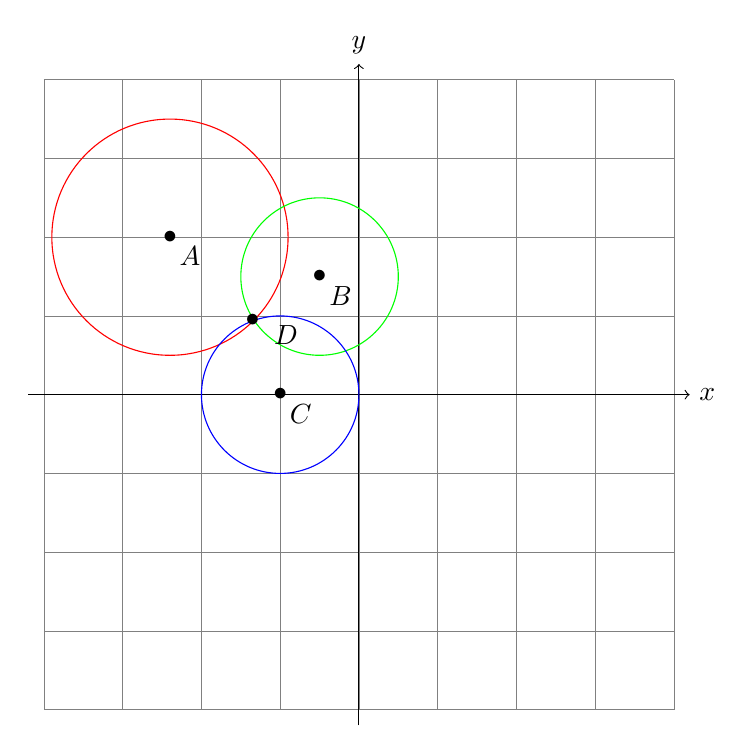
\begin{tikzpicture}
    \draw[very thin,color=gray] (-4,-4) grid (4,4);
    \draw[->] (-4.2,0) -- (4.2,0) node[right] {$x$};
    \draw[->] (0,-4.2) -- (0,4.2) node[above] {$y$};
    
    \draw[color=red] (-2.4,2) circle (1.5);
        \draw (-2.4,2) node {$\bullet$};
        \node[anchor=north west] at (-2.4,2) {$A$};
        
    \draw[color=green] (-0.5,1.5) circle (1);
        \draw (-0.5,1.5) node {$\bullet$};
        \node[anchor=north west] at (-0.5,1.5) {$B$};
        
    \draw[color=blue] (-1,0) circle (1); %2-2sqrt(3)
        \draw (-1,0) node {$\bullet$};
        \node[anchor=north west] at (-1,0) {$C$};
        
    \draw (-1.35,0.95) node {$\bullet$};
    \node[anchor=north west] at (-1.2,1) {$D$};   
\end{tikzpicture}
}
\end{center}
\begin{figure}
\centering
\scalebox{1}{
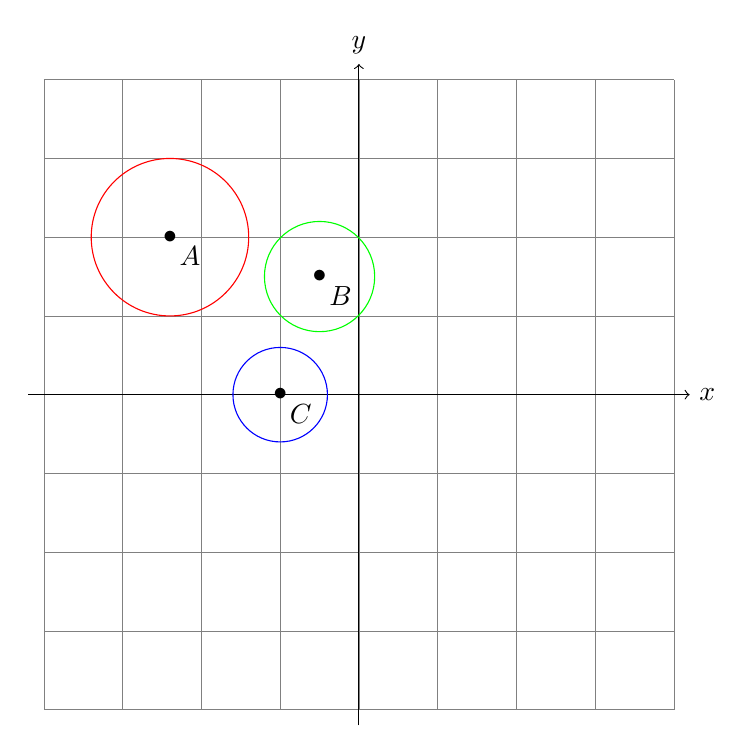
\begin{tikzpicture}
    \draw[very thin,color=gray] (-4,-4) grid (4,4);
    \draw[->] (-4.2,0) -- (4.2,0) node[right] {$x$};
    \draw[->] (0,-4.2) -- (0,4.2) node[above] {$y$};
    
    \draw[color=red] (-2.4,2) circle (1);
        \draw (-2.4,2) node {$\bullet$};
        \node[anchor=north west] at (-2.4,2) {$A$};
        
    \draw[color=green] (-0.5,1.5) circle (0.7);
        \draw (-0.5,1.5) node {$\bullet$};
        \node[anchor=north west] at (-0.5,1.5) {$B$};
        
    \draw[color=blue] (-1,0) circle (0.6); %2-2sqrt(3)
        \draw (-1,0) node {$\bullet$};
        \node[anchor=north west] at (-1,0) {$C$};
\end{tikzpicture}}
\caption{trilKO} \label{fig:trilKO}
\end{figure}

However, this algorithm has many drawbacks. The most important to note is the effect of the noise. Suppose for example to repeat the experiment in a noisy environment, and to obtain a new outcome as in Fig. \ref{fig:trilKO}.

Here there are no intersections, therefore the basic version of this algorithm (without any software level exception catching) would cause a runtime error, and give no results. This problem is overcome by other algorithms, shown later in ?? and ??. Another important drawback is the low number of measurements needed. Indeed, an algorithm that takes few measures is attractive, but the noise cause a not negligible error in the estimated position, that reduces as the number of samples fed to the algorithm increases.
\clearpage

\subsection{Min-max method (intersection of rectangles)}
  \begin{center}
  \textbf{Assume to know:}
  \begin{itemize}
    \centering
    \item $A$
    \item $\alpha$
  \end{itemize}
  \end{center}
  \begin{itemize}
      \item ProblemInvestigationofMin-maxMethodforRSSIbasedIndoorLocalization.pdf
  \end{itemize}
After deriving the distance as shown in ?? of each anchor node from the source, we can draw a circle around each anchor node, which is the locus of points where the target node can be located. Instead of referring to these circles, circumscribe a square to that circle, obtaining a square with side equal to the diameter of the circle. After taking some measurements, you have a set of overlapping squares, close to the representation in fig ??. As a result you can obtain a rectangle with vertices $(x_{min},x_{max},y_{min},y_{max})$ with the following equations:
\begin{equation}
    x_{min}=\max(x_1-d_1,...,x_n-d_n)
\end{equation}
\begin{equation}
    x_{max}=\min(x_1+d_1,...,x_n+d_n)
\end{equation}
\begin{equation}
    y_{min}=\max(y_1-d_1,...,y_n-d_n)
\end{equation}
\begin{equation}
    y_{max}=\min(y_1+d_1,...,y_n+d_n)
\end{equation}
The final location will be estimated as the center of this rectangle, as follows:
\begin{equation}
    x_t=\frac{x_{min}+x_{max}}{2}
\end{equation}
\begin{equation}
    y_t=\frac{y_{min}+y_{max}}{2}
\end{equation}
does it always converge? $x_max$ is always greater than $x_min$?
\clearpage

\subsection{pag 80 book}
  \begin{center}
  \textbf{Assume to know:}
  \begin{itemize}
    \centering
    \item $A$
    \item $\alpha$
    \item $\forall i , 1\leq i\leq n\quad \sigma_{RSS,i}$
  \end{itemize}
  \end{center}
From [handbook of position location zekavat]. Consider this slightly different model, obtained by the canonical one as ??...
\begin{equation}
    RSS_i=-\ln{d_i^{2\frac{\alpha}{2\ln{10}}}}+n_{RSS,i}
\end{equation}
where $\ln$ is the natural logarithm (correct with the base ten the next steps), $n_{RSS,i}$ is the noise, represented as a gaussian random variable with mean $\mu$ and variance $\sigma^2$. Note that $RSS_i=RSSI_i-A$. By taking the inverse of ?? we have 
\begin{equation}
    e^{RSS_i}=e^{-\ln\big(d_i^{2\frac{\alpha}{2}}\big)+n_{RSS,i}}
\end{equation}
\begin{equation}
    \bigg(e^{RSS_i}\bigg)^{-1}=\bigg(e^{-\ln\big(d_i^{2\frac{\alpha}{2}}\big)+n_{RSS,i}}\bigg)^{-1}
\end{equation}
\begin{equation}
    e^{-RSS_i}=e^{\ln\big(d_i^{2\frac{\alpha}{2}}\big)-n_{RSS,i}}
\end{equation}
\begin{equation}
    e^{-RSS_i}=d_i^{2\frac{\alpha}{2}}e^{-n_{RSS,i}}
\end{equation}
\begin{equation}
    \bigg(e^{-RSS_i}\bigg)^{\frac{2}{\alpha}}=\bigg(d_i^{2\frac{\alpha}{2}}e^{-n_{RSS,i}}\bigg)^{\frac{2}{\alpha}}
\end{equation}
\begin{equation}
    e^{-2\frac{RSS_i}{\alpha}}=d_i^2e^{-2\frac{n_{RSS,i}}{\alpha}}
\end{equation}
From \cite{Beran2011} (??spiega tutto il passaggio dai momenti alla media e varianza con dmostrazione...).  Thus if $n\sim\mathcal{N}(\mu,\sigma^2)$ and $c$ a constant then
\begin{equation}
    E[e^n]=e^{\mu+\frac{\sigma^2}{2}}
\end{equation}
\begin{equation}
    E[e^{cn}]=??
\end{equation}
\begin{equation}
Var[e^n]=(e^{\sigma^2}-1)e^{2\mu+\sigma^2}    
\end{equation}
therefore 
\begin{equation}
E\bigg[e^{-2\frac{RSS_i}{\alpha}}\bigg]=d_i^2e^{2\frac{\sigma^2_{RSS,i}}{\alpha^2}}
\end{equation}
\begin{equation}
    Var\bigg[e^{-2\frac{RSS_i}{\alpha}}\bigg]=d_i^4e^{\frac{4\sigma_{RSS_i}^2}{\alpha^2}}\bigg(e^{\frac{4\sigma_{RSS_i}^2}{\alpha^2}}-1\bigg)
\end{equation}
As we can see from ??, $e^{-2\frac{RSS_i}{\alpha}}$ is a biased estimate of $d_i^2$, however we can remove its bias by dividing it by $e^{2\frac{\sigma^2_{RSS,i}}{\alpha^2}}$. Therefore, an unbiased estimate of $d_i^2$ is 
\begin{equation}
    e^{-2\frac{RSS_i}{\alpha}-2\frac{\sigma^2_{RSS,i}}{\alpha^2}}
\end{equation}
We want to use the above estimator obtained from the measurements to build a linear models in $\mathbf{x}$. Since the estimator is now unbiased we can write
\begin{equation}
    (x-x_i)^2+(y-y_i)^2=e^{-2\frac{RSS_i}{\alpha}-2\frac{\sigma^2_{RSS,i}}{\alpha^2}}
\end{equation}
\begin{equation}
    -2x_ix-2y_iy+x^2+y^2+x_i^2+y_i^2=e^{-2\frac{RSS_i}{\alpha}-2\frac{\sigma^2_{RSS,i}}{\alpha^2}}
\end{equation}
\begin{equation}
    -2x_ix-2y_iy+x^2+y^2=e^{-2\frac{RSS_i}{\alpha}-2\frac{\sigma^2_{RSS,i}}{\alpha^2}}-x_i^2-y_i^2
\end{equation}
By calling $R^2=x^2+y^2$ we can write it in matrix form
\begin{equation}
    \begin{bmatrix}
        -2x_1 & -2y_1 & 1\\
        \vdots&\vdots&\vdots\\
        -2x_n & -2y_n & 1
    \end{bmatrix}
    \begin{bmatrix}
        x\\
        y\\
        R^2
    \end{bmatrix} = 
    \begin{bmatrix}
        e^{-2\frac{RSS_1}{\alpha}-2\frac{\sigma^2_{RSS,1}}{\alpha^2}} & -x_1^2 & -y_1^2\\
        \vdots&\vdots&\vdots\\
        e^{-2\frac{RSS_n}{\alpha}-2\frac{\sigma^2_{RSS,n}}{\alpha^2}} & -x_n^2 & -y_n^2\\
    \end{bmatrix}
\end{equation}
with $$M=\begin{bmatrix}
        -2x_1 & -2y_1 & 1\\
        \vdots&\vdots&\vdots\\
        -2x_n & -2y_n & 1
    \end{bmatrix}$$
$$\theta^* =     \begin{bmatrix}
        x\\
        y\\
        R^2
    \end{bmatrix}$$
$$b=    \begin{bmatrix}
        e^{-2\frac{RSS_1}{\alpha}-2\frac{\sigma^2_{RSS,1}}{\alpha^2}} & -x_1^2 & -y_1^2\\
        \vdots&\vdots&\vdots\\
        e^{-2\frac{RSS_n}{\alpha}-2\frac{\sigma^2_{RSS,n}}{\alpha^2}} & -x_n^2 & -y_n^2\\
    \end{bmatrix}$$
Now since $\theta^*$ is unknown we would like to choose $\theta\approx\theta^*$ to have 
\begin{equation}
    M\theta-b\approx0
\end{equation}
One easy way is to find it is to seek the minimum of 
\begin{equation}
    J(\theta)=(M\theta - b)^T(M\theta - b)
\end{equation}
We can fit this model with the Least Square Method, that for a linear model (which is the ours) has a known explicit solution:
\begin{equation}
    \hat{\theta}=(M^TM)^{-1}M^Tb
\end{equation}
the target position can be finally obtained as 
\begin{equation}
\begin{bmatrix}
    \hat{x}\\
    \hat{y}
\end{bmatrix}=
\begin{bmatrix}
    [\hat{\theta}]_1\\
    [\hat{\theta}]_2
\end{bmatrix}
\end{equation}
\clearpage


\subsection{WLLS pag 87 book}
\clearpage


\subsection{NL to Linear transformation pag 410 book}
  \begin{center}
  \textbf{Assume to know:}
  \begin{itemize}
    \centering
    \item $A$
    \item $\alpha$
  \end{itemize}
  \end{center}
From the canonical model extract $d_i$ as follows
\begin{equation*}
    10^{RSSI_{i}}=10^{A-\alpha\log_{10}(d_i)}
\end{equation*}
\begin{equation*}
    10^{RSSI_{i}-A}=10^{-\alpha\log_{10}(d_i)}
\end{equation*}
\begin{equation*}
     10^{RSSI_{i}-A}=d_i^{-\alpha}
\end{equation*}
\begin{equation}
    d_i=10^{\frac{A-RSSI_{i}}{\alpha}}
\end{equation}
so that we have the following set of equations
\begin{align}
\begin{split} 
(x_1-x)^2+(y_1-y)^2&=d_1^2 \\ 
(x_2-x)^2+(y_2-y)^2&=d_2^2 \\ 
&\;\;\vdots\\
(x_n-x)^2+(y_n-y)^2&=d_n^2 \\
\end{split}
\end{align}
Consider 
\begin{align}
\frac{1}{n}&\sum_{i=1}^nd_i^2=\\
&=\frac{1}{n}\sum_{i=1}^n\big[(x_i-x)^2+(y_i-y)^2\big]\\
&=\frac{1}{n}\sum_{i=1}^n(x_i-x)^2+\frac{1}{n}\sum_{i=1}^n(y_i-y)^2\\
&=\frac{1}{n}\sum_{i=1}^n[x_1^2-2x_ix-x^2] + \frac{1}{n}\sum_{i=1}^n[y_1^2-2y_iy-y^2]\\
&=\frac{1}{n}\sum_{i=1}^nx_1^2-2x\frac{1}{n}\sum_{i=1}^nx_i- x^2 + \frac{1}{n}\sum_{i=1}^ny_1^2-2y\frac{1}{n}\sum_{i=1}^ny_i- y^2
\end{align}
By adding ?? to the right member of the previous set of equations and ?? to the left member we have:


\begin{align}
\begin{split} 
    \bigg(x_1-\frac{1}{n}&\sum_{i=1}^nx_i\bigg)x+\bigg(y_1-\frac{1}{n}\sum_{i=1}^ny_i\bigg)y\\
    &=\frac{1}{2}\bigg[\bigg(x_1^2-\frac{1}{n}\sum_{i=1}^nx^2_i\bigg)+\bigg(y_1^2-\frac{1}{n}\sum_{i=1}^ny^2_i\bigg)-\bigg(d_1^2-\frac{1}{n}\sum_{i=1}^nd_i^2\bigg)\bigg]\\
&\;\;\vdots\\
    \bigg(x_n-\frac{1}{n}&\sum_{i=1}^nx_i\bigg)x+\bigg(y_n-\frac{1}{n}\sum_{i=1}^ny_i\bigg)y\\
    &=\frac{1}{2}\bigg[\bigg(x_n^2-\frac{1}{n}\sum_{i=1}^nx^2_i\bigg)+\bigg(y_n^2-\frac{1}{n}\sum_{i=1}^ny^2_i\bigg)-\bigg(d_n^2-\frac{1}{n}\sum_{i=1}^nd_i^2\bigg)\bigg]
\end{split}
\end{align}
So can write the above set of equations in matricial form $\mathbf{Mx}=\mathbf{b}$ by setting
$$
\mathbf{M}=\begin{bmatrix}
    x_1-\frac{1}{n}\sum_{i=1}^nx_i&y_1-\frac{1}{n}\sum_{i=1}^ny_i\\
    \vdots&\vdots\\
    x_n-\frac{1}{n}\sum_{i=1}^nx_i&y_n-\frac{1}{n}\sum_{i=1}^ny_i
\end{bmatrix}
$$
$$
\mathbf{x}=\begin{bmatrix}
    x\\
    y
\end{bmatrix}
$$
$$\mathbf{b}=\frac{1}{2}
\begin{bmatrix}
\bigg(x_1^2-\frac{1}{n}\sum_{i=1}^nx^2_i\bigg)+\bigg(y_i^2-\frac{1}{n}\sum_{i=1}^ny^2_i\bigg)-\bigg(d_i^2-\frac{1}{n}\sum_{i=1}^nd_i^2\bigg)\\
\vdots\\
\bigg(x_n^2-\frac{1}{n}\sum_{i=1}^nx^2_i\bigg)+\bigg(y_n^2-\frac{1}{n}\sum_{i=1}^ny^2_i\bigg)-\bigg(d_n^2-\frac{1}{n}\sum_{i=1}^nd_i^2\bigg)
\end{bmatrix}
$$
then the solution can be computed with the usual Linear Least Square procedure obtaining
\begin{equation}
    \mathbf{x}=(\mathbf{M^TM})^{-1}\mathbf{M^Tb}
\end{equation}




\clearpage
\subsection{line passing between circles pag 385-386 book}

\clearpage

\section{Nonlinear methods}
\subsection{Multilateration}
If you assume to know $A$ then good results with GN method...\\
This algorithm is the generalization of the trilateration method, and is known as multilateration. 
This method can provide two main benefits over the classic trilateration:
\begin{itemize}
    \item Always give a result
    \item The result is made on more observation than the trilateration
\end{itemize}
The first point can be explained as follows:
We start by measuring the rssi value in each position.This measurement can be fitted to the model of $RSSI$ propagation. Assuming that the exact distribution follows 
\begin{equation}
rssi(x,y)=A^*-10\alpha^*\log_{10}\big(\sqrt{(x_t^*-x)^2+(y_t^*-y)^2}\big)    
\end{equation}
with $A^*,\alpha^*,x^*_t,y^*_t$ unknown, we can write a performance index $J$
\begin{equation}
    J(A,n,x_t,y_t)=\sum_{i=1}^n\bigg(rssi_i-A+10\alpha\log_{10}\big(\sqrt{(x_i-x_t)^2+(y_i-y_t)^2}\big)\bigg)
\end{equation}
and then choosing 
\begin{equation}
\Bar{x_t}, \Bar{y_t}=\min_{A,\alpha,x_t,y_t}J(A,\alpha,x_t,y_t)
\end{equation}

\clearpage

\section{Probabilistic approaches}
\begin{itemize}
    \item Maximum Likelihood with covariance weights (improved NLS with the covariance matrix)
    \item Generation of lognormal distribution according to sampled measurements
\end{itemize}
\clearpage

%\section{Statistical supervised Learning techniques} 
%pag 414 415 book	
%\begin{itemize}
%    \item M1
%    \item M2
%\end{itemize}
%\clearpage

\section{Others maybe}
\begin{itemize}
    \item Centroid Algorithm
    \item DV-Hop Algorithm
    \item Fingerprinting
    \item AmorphousAlgorithm
    \item DV-HopMax Algorithm
\end{itemize}

\clearpage





\chapter{Conclusioni (1 pag)}









\clearpage
\printbibliography[
heading=bibintoc,
title={Whole bibliography}
]
%Prints the entire bibliography with the title "Whole bibliography"

\clearpage

%Filters bibliography
\printbibliography[heading=subbibintoc,type=article,title={Articles only}]
%\printbibliography[type=book,title={Books only}]
%\printbibliography[keyword={physics},title={Physics-related only}]
%\printbibliography[keyword={latex},title={\LaTeX-related only}]

\end{document}
